%
% Lösungsverfahren für partielle Differentialgleichungen
%
\section{Lösungsverfahren für lineare partielle Differentialgleichungen}
\kopfrechts{Lösungsverfahren}
Die Wärmeleitungs-, Diffunsions- und Wellengleichungen sind Beispiele
von linearen partiellen Differentialgleichungen.
Die Lösung solcher Gleichungen ist ein eigenes mathematisches
Fachgebiet, hier können daher nur einige wenige Hinweise auf die
grundlegenden Lösungsverfahren gegeben werden.

%
% definitionsgebiet und Randbedingungen
%
\subsection{Definitionsgebiet und Randbedingungen}
%
% fig-gebiet.tex
%
% (c) 2025 Prof Dr Andreas Müller
%
\begin{figure}
\centering
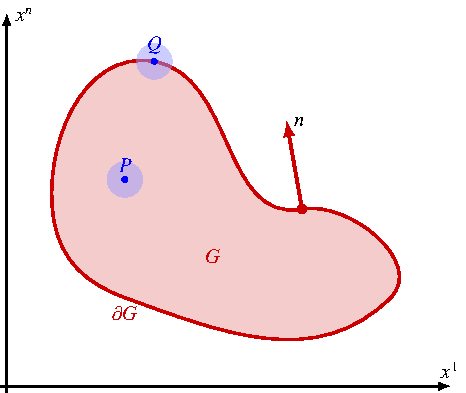
\includegraphics{chapters/080-feldgleichungen/images/gebiet.pdf}
\caption{Gebiet und Rand.
Der Punkt $P$ ist ein innerer Punkt des Gebietes, da es eine kleine
Umgebung gibt, die vollständig in $G$ enthalten ist.
Der Punkt $Q$ ist ein Randpunkt, $Q\in\partial G$, weil jede Umgebung
sowohl Punkte von $G$ wie auch von $\mathbb{R}^n\setminus G$ enthält.
Die Normale $n$ auf den Rand wird zur Definition der Neumann-Randbedingungen
verwendet.
\label{buch:feldgleichungen:loesungsverfahren:fig:gebiet}}
\end{figure}
%
Die Lösung einer partiellen Differentialgleichung ist erst dann vollständig
bestimmt, wenn zusätzlich zur Gleichung geeignete Randbedingungen
vorgegeben werden.

%
% Definitionsgebiet
%
\subsubsection{Definitionsgebiet}
Das Definitionsgebiet kann eine beliebige offene Menge $G\subset\mathbb{R}^n$
sein.
Zur Berechnung partieller Ableitungen einer Funktion in einem Punkt
muss man Funktionswerte in jeder beliebigen Richtung ausgehend von
diesem Punkt auswerten können.
Dies ist nur möglich, wenn es um jeden Punkt von $G$ auch eine kleine
Umgebung gibt, die ebenfalls im Definitionsgebiet der Funktion enthalten
ist.
In Abbildung~\ref{buch:feldgleichungen:loesungsverfahren:fig:gebiet}
ist $P$ ein innerer Punkt des Gebietes $G$.
Nur für solche inneren Punkte ist es sinnvoll zu sagen, dass eine
Funktion die Differentialgleichung erfüllt.

Randbedingungen müssen auf Randpunkten des Gebietes spezifiziert werden.
Dies sind Punkte $x\in\mathbb{R}^n$, für die jede kleine Umgebung sowohl
Punkte von $G$ wie auch ausserhalb von $G$ enthält.
In Abbildung~\ref{buch:feldgleichungen:loesungsverfahren:fig:gebiet}
ist $Q$ ein Randpunkt.
Die Menge der Randpunkte von $G$ wird mit $\partial G$ bezeichnet.
Die Menge $\bar{G}=G\cup \partial G$ enthält sowohl das Gebiet
wie auch die Randpunkte.

Eine Lösung der Differentialgleichung ist eine stetige Funktion
$u\colon\bar{G}\to\mathbb{R}$, die im Inneren, also auf $G$,
genügend oft stetig differenzierbar ist und
die Differentialgleichung erfüllt.
Ausserdem müssen auf einem Teil der Randpunkte zusätzlich
Randbedingungen erfüllt sein.
Da $u$ auch auf dem Rand $\partial G\subset\bar{G}$ definiert
ist, können diese ebenfalls verifiziert werden.

%
% Dirichlet-Randbedingungen
%
\subsubsection{Dirichlet-Randbedingungen}
\index{Dirichlet-Randbedingungen}%
{\em Dirichlet-Randbedingungen} geben Wert der Funktion vor.
Sei also $D\subset\partial G$ eine Teilmenge der Randpunkte
und $g\colon D\to\mathbb{R}$ eine Funktion, dann erfüllt $u$
die Dirichlet-Randbedingung mit den Randwerten $g$, wenn
\[
u(x) = g(x)\qquad \forall x\in D
\]
gilt.

Dirichlet-Randbedingungen liegen im Beispiel der schwingenden Saite
an den Punkten $x=0$ und $x=l$ vor.
Dort sind die Funktionswerte $0$ vorgeben.
Solche Randbedingungen mit Wert 0 werden auch {\em homogenen} 
Randbedingungen genannt.

Die Anfangslage $u(x,0)$ der schwingenden Saite war dagegeben durch
die Funktion $f(x)$ vorgegeben, dies sind Dirichlet-Randbedingungen
auf der Menge $\{(x,0)\mid x\in[0,l]\}$.

\subsubsection{Neumann-Randbedingungen}
\index{Neumann-Randbedingungen}%
{\em Neumann-Randbedingungen} geben statt Funktionswerten die Werte
von Ableitungen vor.
Solche Randwerte können im Allgmeinen die Lösung nicht eindeutig
festlegen, es muss mindestens ein Funktionswert ebenfalls vorgegeben
werden.
Aus einem Funktionswert auf dem Rand und der Ableitung entlang
der Randkurve können durch Integration die Werte auf der Randkurve
ermittelt werden, so dass tatsächlich Dirichlet-Randbedingungen
vorliegen.

Nur Ableitungen senkrecht auf den Rand können tatsächlich neue
Information liefern, die nicht auch durch Dirichlet-Randbedingungen
vorgegeben werden können.
Bezeichnet man mit $n$ die Normale auf den Rand des Gebietes
(Abbildung~\ref{buch:feldgleichungen:loesungsverfahren:fig:gebiet}),
dann wird die Ableitung senkrecht auf den Rand mit
\[
\frac{\partial u}{\partial n}
=
D_n u
\]
bezeichnet und heisst die {\em Normalableitung}.
\index{Normalableitung}%
Neumann-Randbedingungen geben auf einer Teilmenge $N\subset\partial G$
die Normalableitung vor.

Neumann-Randbedingungen lagen im Beispiel der schwingenden Saite bei
der Vorgabe der Anfansgeschwindigkeit
\[
\frac{\partial u}{\partial t}(x,0)
=
g(x)
\]
vor.
Die Ableitung in Richtung $t$ ist die Normalableitung auf dem Randstück
$[0,l]\times \{0\}$ des Randes.

\subsection{Separationsverfahren}
\index{Separationsverfahren}%
Das Verfahren wird am Beispiel der Wellengleichung
\eqref{buch:feldgleichungen:wellengleichung:eqn:wellengleichung}
in der eindimensionalen Form
\begin{equation}
\frac{\partial^2 u}{\partial t^2}
=
a^2
\frac{\partial^2 u}{\partial x^2}
\label{buch:feldgleichungen:loesung:eqn:wellengleichung}
\end{equation}
illustriert.
Es funktioniert, wenn das Gebiet $G$ auf dem die Funktion $u$
definiert ist, ein Rechteck ist.
Für den vorliegenden Fall nehmen wir an, dass $u$ auf
$[0,l]\times\mathbb{R}$ definiert ist, und dass an den
Intervall-Enden homogene Dirichlet-Randbedingungen der Form 
\[
u(0,t)=u(l,t)=0
\]
gegeben sind.
Neumann-Randbedingungen können auf analoge Art behandelt werden.

Wir nehmen an, dass sich die Lösung als Produkt $u(x,t)=X(x)T(t)$
von zwei Funktionen schreiben, wobei $X$ nur von $x$ und $T$ nur
von $t$ abhängt.
Durch Einsetzen des Ansatzes in
\eqref{buch:feldgleichungen:loesung:eqn:wellengleichung} 
ist
\[
T''(t) X(x)
=
a^2
T(t)
X''(x).
\]
Nach Division durch $u$ lassen sich die nicht abgeleiteten Faktoren
kürzen und es bleibt
\begin{equation}
\frac{T''(t)}{T(t)}
=
a^2
\frac{X''(x)}{X(x)}.
\label{buch:feldgleichungen:loesung:eqn:separiert}
\end{equation}
Die linke Seite hängt nur von $t$ ab, während die rechte nur von $x$
abhängt.
Man sagt, die Variablen sind {\em separiert} worden.
Die Gleichung~\eqref{buch:feldgleichungen:loesung:eqn:separiert}
kann nur erfüllt werden, wenn beide Seiten konstant sind.
Es gibt daher eine Konstante $\lambda$, mit der sich die
Gleichung~\eqref{buch:feldgleichungen:loesung:eqn:separiert}
in die zwei Gleichungen
\[
\begin{aligned}
\frac{T''(t)}{T(t)}&=\lambda &&\Rightarrow& T''(t) &= \lambda T(t) \\
\frac{X''(x)}{X(x)}&=\lambda &&\Rightarrow& X''(x) &= \lambda X(x)
\end{aligned}
\]
zerlegen lässt.
Dies sind gewöhnliche Differentialgleichungen, die sich unabhängig
voneinander lösen lassen.

Für $\lambda > 0$ wachsen die Lösungen exponentiell schnell an, was
nicht dem Verhalten einer Welle entspricht.
Wir dürfen daher annehmen, dass $\lambda \le 0$ ist und schreiben
$\lambda = -k^2$ mit $k\in\mathbb{R}$, um dies sicherzustellen.
Die Differentialgleichungen bekommen daher die Form
\begin{align*}
X''(x) &= -k^2 X(x)
&&\text{und}&
T''(t) &= -k^2 T(t),
\intertext{die die Lösungen}
X(x) &= A\cos kx + B \sin kx
&&\text{und}&
T(t) &= A\cos kt + B \sin kt
\end{align*}
haben.

Für die Bestimmung der Koeffizienten $A$ und $B$ müssen die 
Randbedingungen hinzugezogen werden.
Dies können nicht für jeden Wert von $k$ erfüllt werden.
Die homogenen Randbedingungen für $X(x)$ verlangen, dass
\begin{equation*}
\left.
\bgroup
\renewcommand{\arraycolsep}{1pt}
\begin{array}{rlcrlcl}
A&\cos 0 &\,+\,&B&\sin 0  &\,=\,& 0\\
A&\cos kl&\,+\,&B&\sin kl &\,=\,& 0
\end{array}
\egroup
\quad
\right\}
\qquad\Rightarrow\qquad
\left\{
\quad
\begin{aligned}
        A&= 0 \\
B\sin kl &= 0
\end{aligned}
\right.
\end{equation*}
Da $B=0$ nur die Null-Lösung ergäbe, muss $\sin kl=0$ sein, was nur
dann möglich ist, wenn $kl$ ein Vielfaches von $\pi$ ist.
Es gibt also eine natürliche Zahl $n$ derart, dass
$kl=n\pi$ und daher $k=n\pi/l$.
Die Randbedingungen legen daher fest, dass für jedes natürlich $n$ eine
Lösung
\[
X(x) = B \sin \frac{n\pi x}{l}
\qquad\text{und}\qquad
T(t) = A \cos \frac{n\pi t}{l} + B \sin\frac{n\pi t}{l}
\]
gefunden werden kann.

Dank der Linearität der Gleichung kann die allgemeine Lösung der
Wellengleichung jetzt durch die Überlagerung
\[
u(x,t)
=
\sum_{n=1}^\infty
\biggl(
a_n\cos\frac{n\pi t}{l}
+
b_n\sin\frac{n\pi t}{l}
\biggr)
\sin\frac{n\pi x}{l}
\]
konstruiert werden, deren Koeffizienten $a_n$ und $b_n$ durch
Heranziehen weitere Randbedingungen bestimmt werden müssen.

Seien jetzt zusätzlich Dirichlet- und Neumann-Randbedingungen zur Zeit
$t$ gegeben.
Es gibt daher Funktionen $f(x)$ und $g(x)$, die
\[
\renewcommand{\arraycolsep}{2pt}
\begin{array}{rclcl}
u(x,0)
&=&
\displaystyle
\sum_{n=0}^\infty \phantom{\frac{n\pi}{l}}a_n \sin\frac{n\pi x}{l}
&=&
f(x) \\
\displaystyle
\frac{\partial u}{\partial t}(x,0)
&=&
\displaystyle
\sum_{n=0}^\infty \frac{n\pi}{l}b_n \sin\frac{n\pi x}{l}
&=&
g(x).
\end{array}
\]
Zur Bestimmung der Koeffizienten $a_n$ und $b_n$ müssen wir die
Funktionen $f$ und $g$ in eine Fourier-Sinusreihe
\begin{align*}
f(x) & = \sum_{n=1}^\infty b_n(f)\sin \frac{n\pi x}{l} \\
g(x) & = \sum_{n=1}^\infty b_n(g)\sin \frac{n\pi x}{l}
\end{align*}
entwickeln.
Dann können die Koeffizienten durch Koeffizientenvergleich gefunden
werden.
Die Lösung ist dann
\[
u(x,t)
=
\sum_{n=1}^\infty
\biggl(
b_n(f)
\cos\frac{n\pi t}{l}
+
\frac{lb_n(g)}{n\pi}
\sin\frac{n\pi t}{l}
\biggr)
\sin\frac{n\pi x}{l}.
\]

\subsection{Transformationsverfahren}
\index{Transformationsverfahren}%
Die Lösung der Wellengleichung mit dem Separationsverfahren hat 
auf ganz natürlich Art und Weise auf Fourier-Reihen geführt.
So hat auch Joseph Fourier im 19.~Jahrhundert die nach ihm benannten
Reihen entdeckt.
Es liegt daher nahe zu vermuten, dass sich partielle Differentialgleichungen
auch lösen lassen, indem man sie einer Integraltransformation
unterwirft.
Wir illustrieren dies am Beispiel der Wärmeleitung in einem 
an den Enden isolierten Stab.

Wir betrachten die Differentialgleichung
\[
\frac{\partial T}{\partial x}
=
\kappa
\frac{\partial^2 T}{\partial x^2}
\]
auf dem Gebiet $[0,\pi]\times\mathbb{R}^+$, wobei wir das Intervall
vor allem deshalb gewählt haben, weil sich damit später einfachere
Formeln ergeben.
Ausserdem werden homogene Neumann-Randbedingungen an den
Intervallenden angenommen.
Dies bedeutet, dass die Ableitungen nach $x$ an den Intervallenden
verschwinden, was physikalisch bedeutet, dass kein Wärmeaustausch
über die Enden des Stabes erfolgt.
Ausserdem wird die Temperaturverteilung $T(x)=T(x,0)$ zur Zeit $t=0$
vorgegeben.

Da die Ableitung von $u$ nach $x$ für $x=0$ und $x=\pi$ verschwinden
muss, kann man die Funktion $x\mapsto u(x,t)$ zu einer in $x$
geraden Funktion auf dem Intervall $[-\pi,\pi]$ ausdehnen, die
man ihrerseits zu einer $2\pi$-periodischen Funktion erweitern kann.
Somit muss es eine Entwicklung der Funktion $T(x,t)$ in
eine Fourier-Kosinusreihe
\[
T(x,t)
=
\frac{a_0(t)}{2}
+
\sum_{n=1}^\infty
a_n(t) \cos nx
\]
geben.
Setzt man sie in die Wärmeleitungsgleichung ein, erhält man
\[
\frac{\dot{a}_0}{2}
+
\sum_{n=1}^\infty
\dot{a}_n(t) \cos nx
=
-
\kappa
\sum_{n=1}^\infty
n^2
\cos nx.
\]
Durch Koeffizientenvergleich findet man die gewöhnlichen
Differentialgleichungen
\begin{align}
\dot{a}_0(t)&=0
&&\text{und}&
\dot{a}_n(t)&=-n^2 a_n(t).
\label{buch:feldgleichungen:loesungen:transformation:ode}
\end{align}
Zur Lösung dieser Differentialgleichungen werden zusätzlich
Anfangsbedingungen benötigt, die man aus der Entwicklung der
Funktion $T(x)$ in eine Fourier-Kosinusreihe gewinnen kann.
\index{Fourier-Kosinusreihe}%
Aus 
\[
T(x)
=
\frac{A_0}2
+
\sum_{n=1}^\infty A_n \cos nx
\]
kann man ablesen, dass
\begin{align*}
a_0(0) &= A_0
&&\text{und}&
a_n(0) &= A_n
\end{align*}
sein muss.
Damit kann man jetzt die Lösung der Differentialgleichungen
\eqref{buch:feldgleichungen:loesungen:transformation:ode}
finden.
Die erste Differentialgleichung sagt, dass $a_0(t)=A_0$ konstant ist.
Die zweite Differentialgleichung sagt, dass $a_n(t) = A_ne^{-n^2t}$
sein muss.
Daraus lässt sich die Lösung als
\[
T(x,t)
=
\frac{A_0}{2}
+
\sum_{n=1}^\infty
A_n
e^{-n^2t}
\cos nx
\]
zusammensetzen.

